\documentclass[UTF8,zihao=-4]{ctexart}
\usepackage[a4paper,margin=2.5cm]{geometry}
\usepackage{amsmath, amssymb, amsthm}
\usepackage{bm}
\usepackage{hyperref}
\usepackage{graphicx}
\usepackage{caption}
\usepackage{listings}
\usepackage{xcolor}
\usepackage{float}
\usepackage{booktabs}
\usepackage{longtable}
\usepackage{multirow}
\usepackage{placeins}
\graphicspath{{figures/}}

% 代码样式
\lstdefinestyle{code}{
  basicstyle=\ttfamily\small,
  numbers=left,
  numberstyle=\tiny,
  numbersep=8pt,
  keywordstyle=\color{blue},
  commentstyle=\color{teal!70!black},
  stringstyle=\color{orange!70!black},
  showstringspaces=false,
  breaklines=true,
  frame=single,
  framerule=0.3pt,
  rulecolor=\color{black!15}
}
\lstset{style=code}

\title{多智能体系统:架构拆解、框架生态与行业落地}
\author{}
\date{\today}

\begin{document}
\maketitle

\section{智能体结构:Planner / Executor / Memory / Tool}
\subsection{层次化架构}
成熟的多智能体系统通常遵循规划器(Planner)、执行器(Executor)、记忆模块(Memory)与工具层(Tooling Layer)的分层设计。图\ref{fig:multi_agent_architecture} 展示了典型的信号流:规划器负责任务拆解与策略生成;执行器调用工具完成原子行为;记忆模块在短期/长期之间同步状态;工具层与外部环境交互。
\begin{figure}[H]
  \centering
  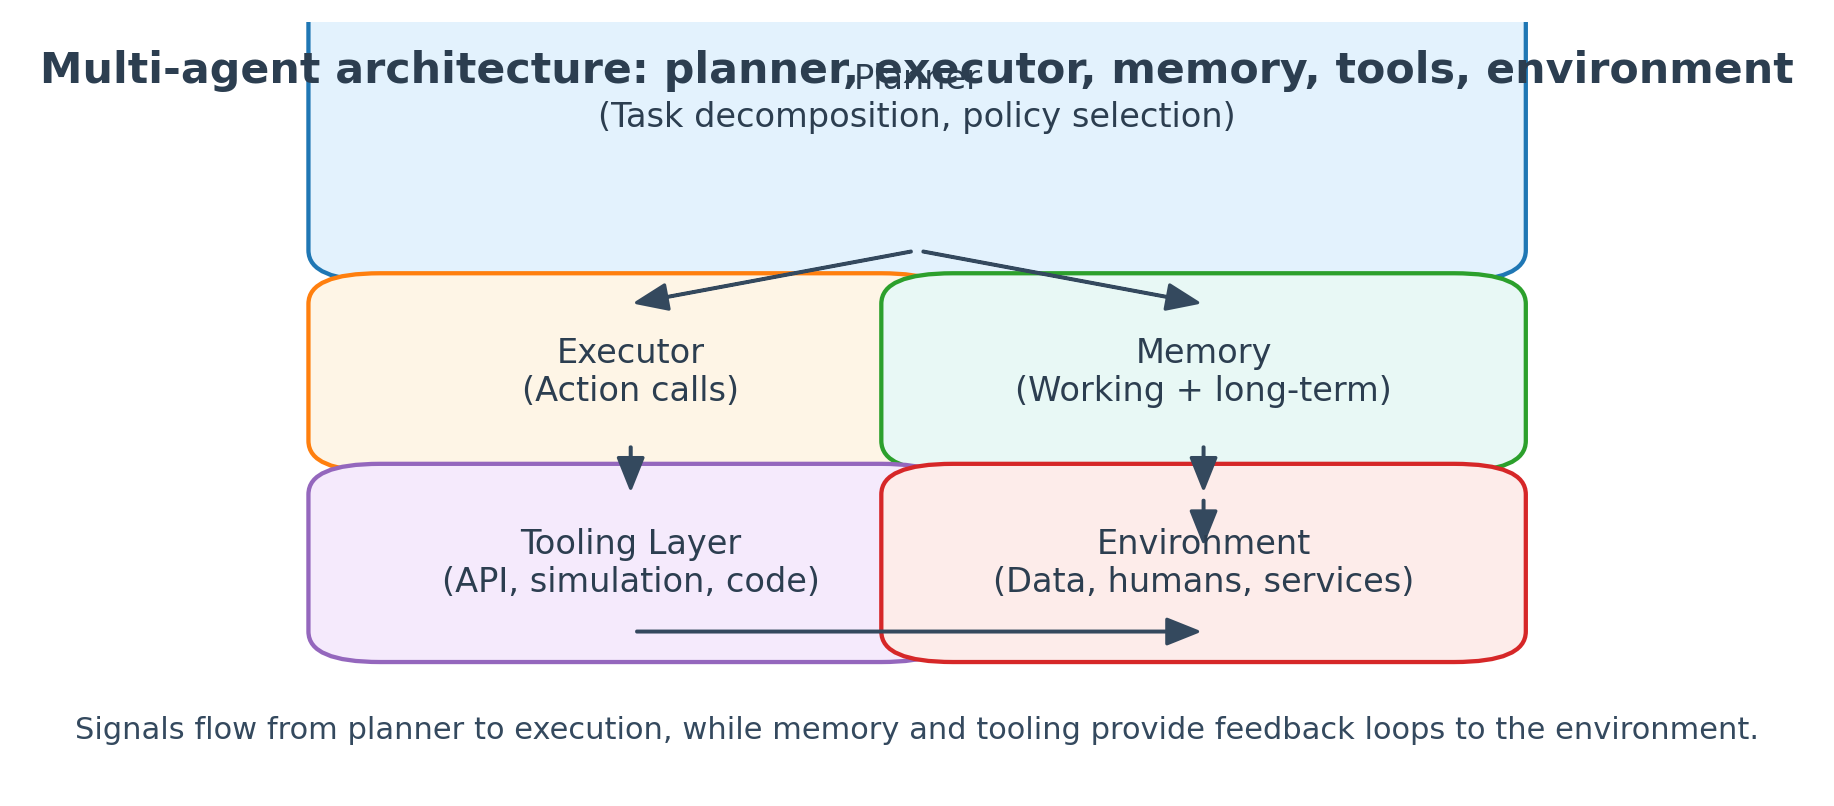
\includegraphics[width=0.95\textwidth]{multi_agent_architecture.png}
  \caption{多智能体架构:规划、执行、记忆、工具与环境之间的协同。}
  \label{fig:multi_agent_architecture}
\end{figure}

\subsection{模块职责}
\begin{itemize}
  \item \textbf{Planner:} 根据用户目标、上下文记忆和外部约束生成多步计划;对复杂任务可结合树搜索、Large Action Model(LAM)策略。
  \item \textbf{Executor:} 负责具体行动的调度与执行,例如 API 调用、脚本运行、自然语言交互。常结合 ReAct 模式输出 Thought/Action/Observation。
  \item \textbf{Memory:} 包含短期工作记忆(Working Memory)与长期知识库(Long-term Memory)。常使用向量数据库、知识图谱或事件日志。
  \item \textbf{Tooling Layer:} 封装外部工具(代码执行、检索服务、仿真环境、数据接口),提供统一的调用协议与权限控制。
  \item \textbf{Environment:} 包括真实世界系统、用户、数据库等,需要进行权限校验、速率限制与错误恢复。
\end{itemize}

\subsection{设计要点}
\begin{itemize}
  \item \textbf{闭环反馈:} 执行结果、环境反馈需要即时返回 Planner 调整后续行动,形成 sense-plan-act 循环。
  \item \textbf{安全控制:} 对工具调用设置权限、白名单、参数验证;通过审计日志追踪操作。
  \item \textbf{多模态能力:} 当涉及图像/语音时,在工具层加入多模态编码器,将结果写入 Memory 供 Planner 决策。
\end{itemize}

\section{LangChain、CrewAI、AutoGPT 框架}
\subsection{框架生态概览}
\begin{longtable}{p{3cm}p{4.5cm}p{6cm}}
\toprule
框架 & 核心特点 & 适用场景 \\
\midrule
LangChain & 模块化链式组合、AgentExecutor、Memory、Tool 接口丰富;社区生态完善 & 快速原型、业务流程自动化、与传统系统集成 \\
CrewAI & 面向多代理协作,提供角色分工、任务队列、同步/异步调度 & 团队型工作流(如内容制作、知识库构建) \\
AutoGPT & 自主目标探索,支持长记忆、文件系统、插件化工具 & 自主研究、脚本生成、实验探索(需额外安全控制) \\
\bottomrule
\end{longtable}

\subsection{LangChain AgentExecutor 示例}
\begin{lstlisting}[language=Python,caption={LangChain 基于 Planner-Executor 模式的 Agent}]
from langchain.agents import initialize_agent, AgentType, Tool
from langchain.chat_models import ChatOpenAI
from langchain.memory import ConversationBufferMemory
import requests

def search_api(query: str) -> str:
    resp = requests.get("https://api.serpapi.com/search", params={"q": query, "api_key": "KEY"})
    return resp.json().get("organic_results", [])

tools = [
    Tool(
        name="web_search",
        func=lambda q: str(search_api(q)[:3]),
        description="Use this when you need to find recent information on the web."
    )
]

llm = ChatOpenAI(model="gpt-4o-mini", temperature=0)
memory = ConversationBufferMemory(memory_key="chat_history", return_messages=True)

agent = initialize_agent(
    tools=tools,
    llm=llm,
    agent=AgentType.CONVERSATIONAL_REACT_DESCRIPTION,
    memory=memory,
    verbose=True,
)

result = agent.run("Summarize the latest breakthroughs in geothermal inversion.")
print(result)
\end{lstlisting}

\subsection{CrewAI 协作模式}
\begin{itemize}
  \item 使用 \texttt{Crew} 定义团队,包含多个 Agent(Writer、Reviewer、Researcher),每个 Agent 绑定工具和记忆;
  \item 支持同步和异步调度:同步队列适用于严格流程,异步模式可提升吞吐;
  \item 集成任务板(Task Board)记录任务状态,便于监控与回溯。
\end{itemize}

\subsection{AutoGPT 与自托管}
AutoGPT 将 LLM 与本地执行环境结合,可持续生成目标、分解任务、执行命令。部署时需注意:
\begin{itemize}
  \item 设置 \texttt{ALLOWLISTED\_COMMANDS} 与工作目录,避免破坏性操作;
  \item 结合安全代理(Guard Agent)审核指令;
  \item 对记忆模块(如向量库、本地文件)设置配额与清理机制。
\end{itemize}

\section{自主任务规划与多代理协作}
\subsection{协作拓扑}
图\ref{fig:agent_collaboration} 展示了多代理协作的常见角色:研究代理负责资料搜索,代码代理构建流水线,分析代理评估结果,内存中心与编排器在中间协调信息与决策。
\begin{figure}[H]
  \centering
  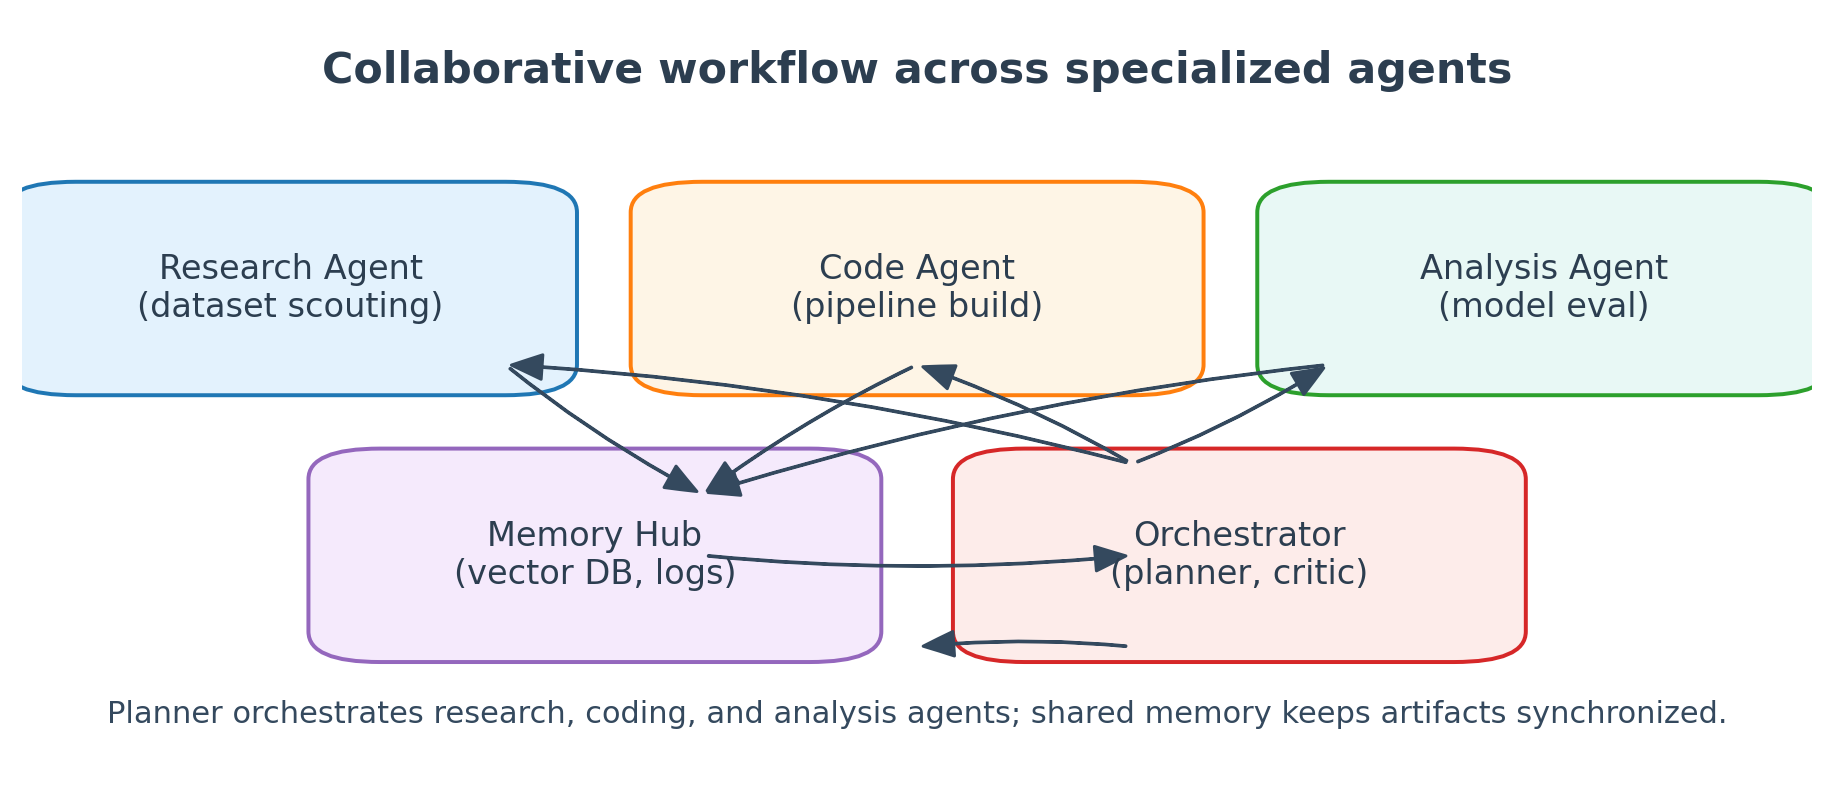
\includegraphics[width=0.95\textwidth]{agent_collaboration.png}
  \caption{多代理协作流程:共享记忆、编排器与专业化智能体的交互。}
  \label{fig:agent_collaboration}
\end{figure}

\subsection{任务规划策略}
\begin{itemize}
  \item \textbf{分层规划:} 高层规划器决定阶段目标,子规划器针对具体任务生成行动序列;
  \item \textbf{自适应调度:} 根据执行结果动态调整队列优先级,使用奖励模型评估代理贡献;
  \item \textbf{共识机制:} 通过辩论(Debate)、投票或裁判 Agent 确认最终答案,降低幻觉风险;
  \item \textbf{冲突处理:} 当多个 Agent 同时修改资源时,使用锁/事务或乐观并发策略。
\end{itemize}

\subsection{协作范式}
\begin{itemize}
  \item \textbf{流水线模式:} 各 Agent 串行完成任务,适合明确流程(如报告生成);
  \item \textbf{黑板模式:} Agent 在共享黑板发布/订阅任务状态,适合科研探索;
  \item \textbf{市场模式:} Agent 根据成本/收益竞价任务,适用于资源抢占型系统;
  \item \textbf{联盟模式:} Agent 组成小组协同完成子任务,并设定内部角色。
\end{itemize}

\subsection{指标与评估}
\begin{longtable}{p{3cm}p{3cm}p{4cm}p{4cm}}
\toprule
指标类别 & 代表指标 & 关注点 & 监控方式 \\
\midrule
效率 & 平均任务完成时间、吞吐量 & 调度是否合理 & Prometheus、Grafana \\
质量 & 用户评分、专家审核、自动评分器 & 结果准确性与可解释性 & GPT Judge、质量对齐模型 \\
协作 & 通信频率、冲突率、成功协同次数 & 协同成本与收益 & 日志分析、事件回放 \\
安全 & 拒绝率、异常命令数、权限违规 & 风险控制效果 & 审计日志、策略引擎 \\
\bottomrule
\end{longtable}

\section{实际应用:科研、代码生成、地球物理解释}
\subsection{科研助理}
\begin{itemize}
  \item \textbf{文献调研:} 研究 Agent 调用学术搜索 API,归档摘要并写入向量记忆,规划器安排后续阅读与问题生成;
  \item \textbf{实验设计:} 代码 Agent 自动生成实验脚本、配置文件,执行结果日志写入 Memory 供分析 Agent 复盘;
  \item \textbf{论文起草:} Writer Agent 根据记忆汇总段落,Reviewer Agent 校验引用、检测重复。
\end{itemize}

\subsection{代码生成与维护}
\begin{itemize}
  \item \textbf{需求理解:} Planner 将需求拆解为模块,代码 Agent 逐个实现并运行单元测试;
  \item \textbf{安全审计:} Security Agent 检查潜在漏洞,工具层集成静态分析器;
  \item \textbf{持续集成:} DevOps Agent 与 CI/CD 工具交互,更新部署状态并记录回滚步骤。
\end{itemize}

\subsection{地球物理解释}
\begin{itemize}
  \item \textbf{数据显示:} 数据 Agent 连接地震/地磁数据库,执行预处理、异常检测;
  \item \textbf{模型推断:} 反演 Agent 调用高性能计算工具运行地球物理反演模型;
  \item \textbf{结果分析:} 解释 Agent 输出地质结构描述、置信度、与历史案例对比;
  \item \textbf{专家监督:} 人类专家通过审阅界面确认结果、修改参数并反馈给系统。
\end{itemize}

\section*{实践建议}
\begin{itemize}
  \item 将多智能体任务拆解为清晰的角色与接口,采用结构化协议(JSON schema)约束通信。
  \item 引入治理机制:包括人类审查回路(Human-in-the-loop)、权限隔离、沙箱执行。
  \item 构建统一的日志与可观测性平台,实现事件回放、性能分析与安全审计。
  \item 在上线前通过对抗测试(红队)评估系统鲁棒性,确保协作过程可控可解释。
\end{itemize}

\section*{参考文献}
\begin{itemize}
  \item Wang et al. ``Voyager: An Open-Ended Embodied Agent with Large Language Models.'' arXiv, 2023.
  \item Shinn et al. ``Reflexion: Language Agents with Verbal Reinforcement Learning.'' NeurIPS, 2023.
  \item Park et al. ``Generative Agents: Interactive Simulacra of Human Behavior.'' SIGGRAPH, 2023.
  \item Qian et al. ``AutoGen: Enabling Next-Gen LLM Applications via Multi-Agent Conversations.'' Microsoft Research, 2023.
  \item Arora et al. ``CrewAI: Orchestrating Collaborative AI Workers.'' arXiv, 2024.
\end{itemize}

\end{document}

